\chapter{SYSTEM DESIGN AND IMPLEMENTATION}

\section{System Overview}

TinkerBlocks is a comprehensive educational system that integrates computer vision, robotics, and mobile technology to create an intuitive programming learning environment. Children arrange physical programming blocks on a grid, and the system uses real-time computer vision to recognize these arrangements and execute them on a robotic car.

The system consists of four main integrated components:
\begin{enumerate}
    \item \textbf{Physical Programming Interface}: Grid board with blocks representing programming commands
    \item \textbf{Raspberry Pi Control System}: Computer vision processing and command interpretation
    \item \textbf{Robotic Car}: Arduino-controlled vehicle with sensors and actuators
    \item \textbf{Mobile Application}: Real-time communication and system monitoring
\end{enumerate}
\begin{figure}[H]
    \centering
    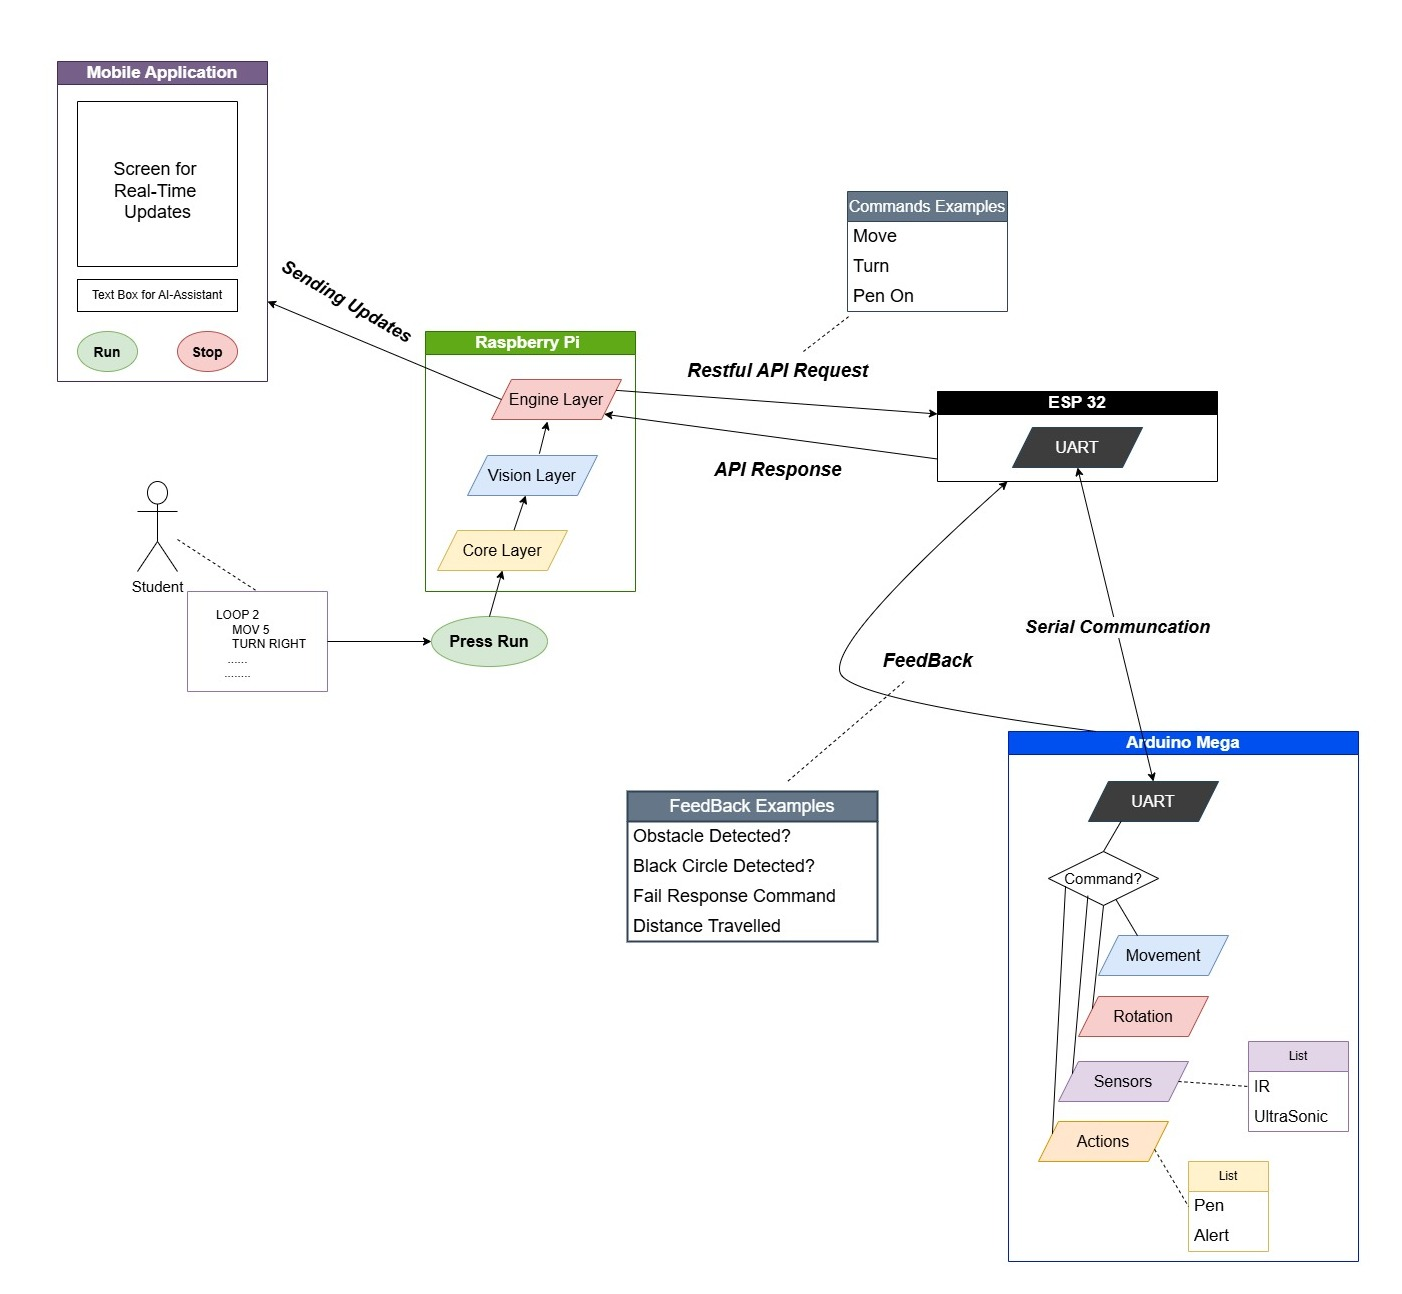
\includegraphics[width=0.9\textwidth]{assets/system_design.jpg}
    \caption{Complete System Communication Flow and Component Integration}
    \label{fig:system_design}
\end{figure}
\begin{figure}[H]
    \centering
    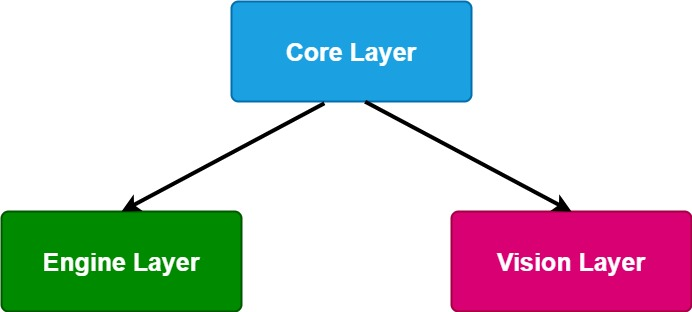
\includegraphics[width=0.8\textwidth]{assets/System_Arch.jpg}
    \caption{Raspberry Pi Software Architecture - Core, Vision, and Engine Modules}
    \label{fig:raspberry_pi_architecture}
\end{figure}

\section{System Architecture}

The TinkerBlocks architecture follows a distributed, modular design that enables real-time communication between multiple specialized components.

\subsection{Distributed Component Architecture}

\textbf{Raspberry Pi Hub}: Serves as the central intelligence, running three specialized modules:
\begin{itemize}
    \item \textbf{Core Module}: WebSocket server, process control, and configuration management
    \item \textbf{Vision Module}: Camera capture, OCR processing, and grid mapping
    \item \textbf{Engine Module}: Command interpretation and program execution logic
\end{itemize}

\textbf{Arduino Car Controller}: Handles direct hardware control with sophisticated firmware:
\begin{itemize}
    \item Class-based architecture for motor control, sensor management, and movement algorithms
    \item Real-time sensor processing and feedback control systems
    \item Serial API for communication with ESP32 bridge
\end{itemize}

\textbf{ESP32 WiFi Bridge}: Provides wireless communication between Raspberry Pi and Arduino:
\begin{itemize}
    \item HTTP REST API server for remote car control
    \item Serial communication bridge to Arduino
    \item JSON protocol translation between HTTP and serial interfaces
\end{itemize}

\textbf{Mobile Application}: React Native interface for user interaction:
\begin{itemize}
    \item WebSocket communication with Raspberry Pi
    \item Real-time chat interface and system control
    \item Cross-platform compatibility for iOS and Android
\end{itemize}

\subsection{Communication Flow}

The system operates through a complete workflow:
\begin{enumerate}
    \item Children arrange programming blocks on the physical grid
    \item Camera captures the grid arrangement
    \item Computer vision processes the image and extracts block positions and text
    \item Command interpreter translates the visual program into executable commands
    \item Commands are sent via WebSocket to ESP32, then via serial to Arduino
    \item Arduino executes commands while providing sensor feedback
    \item Mobile app displays real-time status and execution progress
\end{enumerate}

\section{Hardware Design and Implementation}

\subsection{Robotic Car}

The robotic car serves as the primary execution platform, designed for precision, reliability, and educational engagement.

\begin{figure}[H]
    \centering
    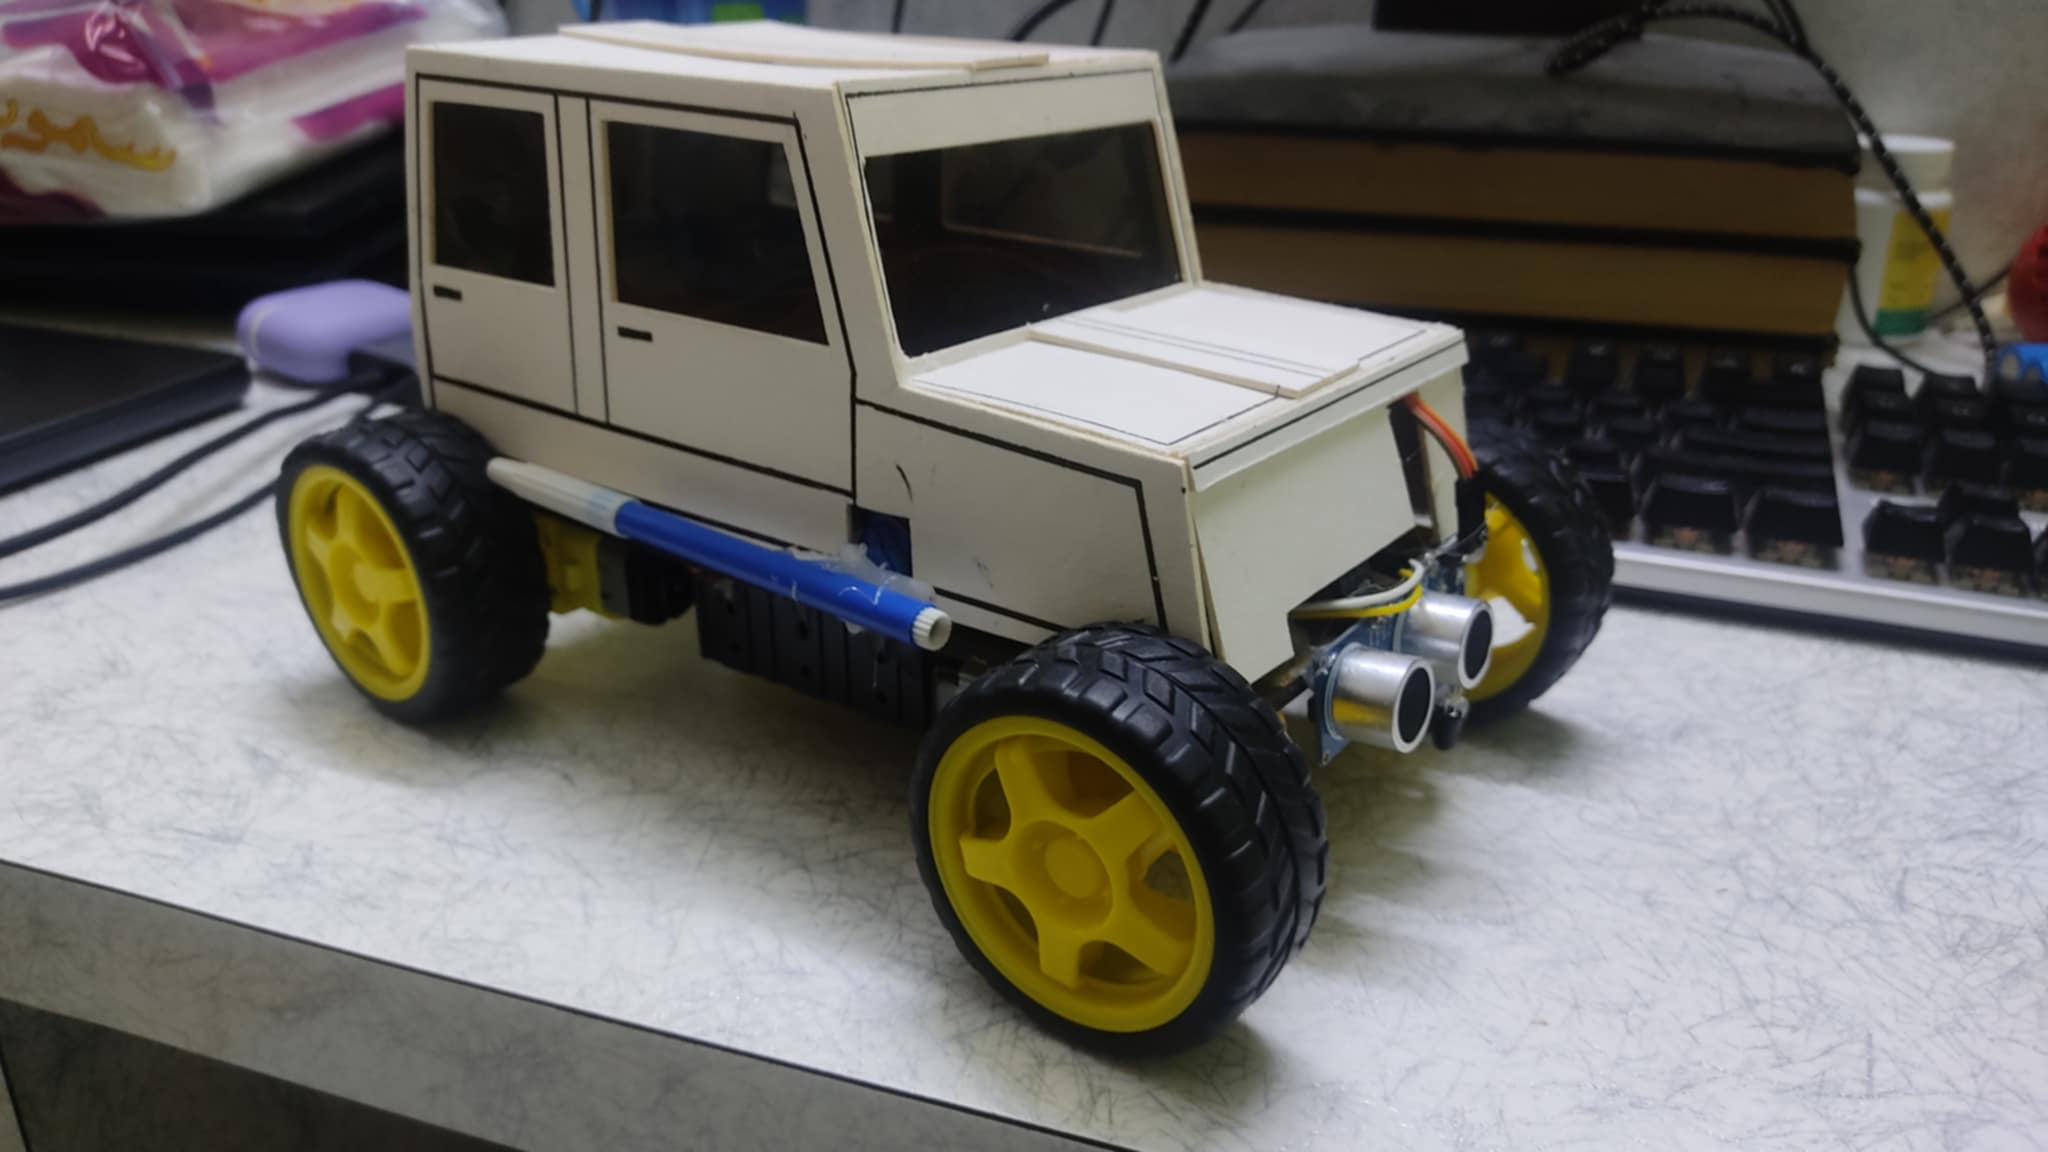
\includegraphics[width=0.7\textwidth]{assets/car.png}
    \caption{TinkerBlocks Robotic Car - Complete Assembly}
    \label{fig:car_complete}
\end{figure}

\subsubsection{Mechanical Design}
\begin{itemize}
    \item \textbf{Chassis}: Custom wooden frame (10cm × 20cm) for durability and cost-effectiveness
    \item \textbf{Propulsion}: Four DC motors with differential steering (tank-style turning)
    \item \textbf{Motor Control}: Two H-bridge modules controlling motor pairs
    \item \textbf{Weight Distribution}: Balanced design for stable movement and turning
\end{itemize}

\subsubsection{Electronic Systems}
\textbf{Primary Controller - Arduino Mega 2560}:
\begin{itemize}
    \item Manages all sensors, motors, and actuators
    \item Implements sophisticated movement algorithms with sensor feedback
    \item Provides comprehensive serial API for external control
    \item Handles real-time control loops for precise movement
\end{itemize}

\textbf{WiFi Communication - ESP32}:
\begin{itemize}
    \item Exposes HTTP REST API for wireless car control
    \item Bridges between WiFi commands and Arduino serial interface
    \item Handles JSON protocol translation and error management
    \item Provides reliable communication with timeout and retry mechanisms
\end{itemize}

\textbf{Power Management}:
\begin{itemize}
    \item Three 3.7V lithium-ion batteries providing 11.1V total
    \item Voltage regulator stepping down to 5V for Arduino and logic circuits
    \item Approximately 2-3 hours of continuous operation
    \item Battery monitoring and protection circuits
\end{itemize}

\subsubsection{Sensor Integration}
\textbf{Navigation and Orientation}:
\begin{itemize}
    \item \textbf{MPU-6050}: 6-axis gyroscope and accelerometer for precise orientation tracking
    \item \textbf{Yaw Correction}: Gyroscope-based straight-line movement compensation
    \item \textbf{PID Control}: Feedback-controlled rotation for accurate turning angles
\end{itemize}

\textbf{Environmental Sensing}:
\begin{itemize}
    \item \textbf{HC-SR04 Ultrasonic Sensor}: Front-mounted obstacle detection with configurable thresholds
    \item \textbf{IR Sensors}: Black line detection for boundary sensing and target recognition
    \item \textbf{Real-time Processing}: Continuous sensor monitoring during movement
\end{itemize}

\textbf{Interactive Features}:
\begin{itemize}
    \item \textbf{Servo-Controlled Pen}: Precision drawing mechanism for creative programming tasks
    \item \textbf{Position Tracking}: Coordinate system for drawing and navigation
    \item \textbf{Path Recording}: Movement history for visualization and debugging
\end{itemize}

\subsection{Programming Grid Interface}

\subsubsection{Physical Structure}
\begin{itemize}
    \item \textbf{Grid Configuration}: 16 columns × 10 rows (configurable for different complexity levels)
    \item \textbf{Block Placement}: Physical holes for precise block positioning and stability
    \item \textbf{Material}: Durable wooden construction suitable for classroom use
    \item \textbf{Portability}: Lightweight design for easy setup and storage
\end{itemize}

\begin{figure}[H]
    \centering
    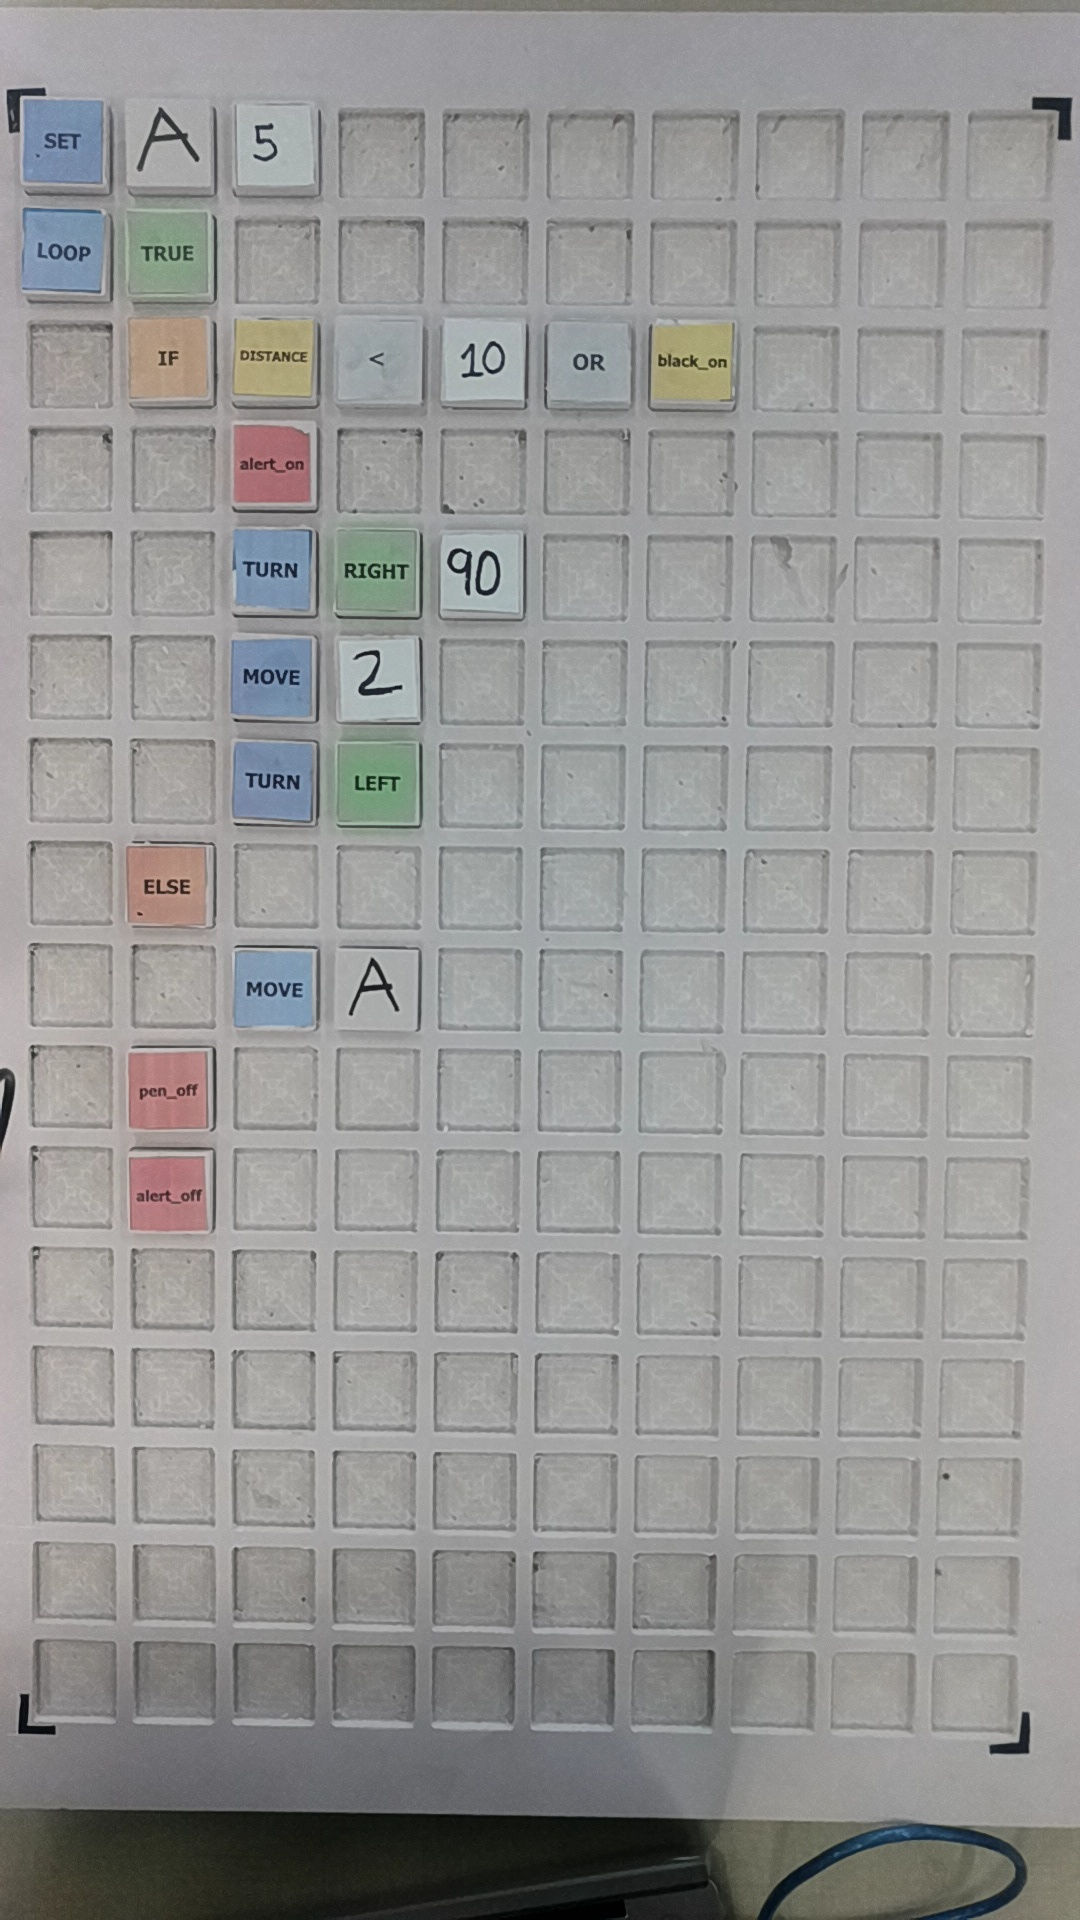
\includegraphics[width=0.6\textwidth]{assets/board.jpg}
    \caption{Programming Grid with Sample Block Arrangement}
    \label{fig:programming_grid}
\end{figure}

\begin{figure}[H]
    \centering
    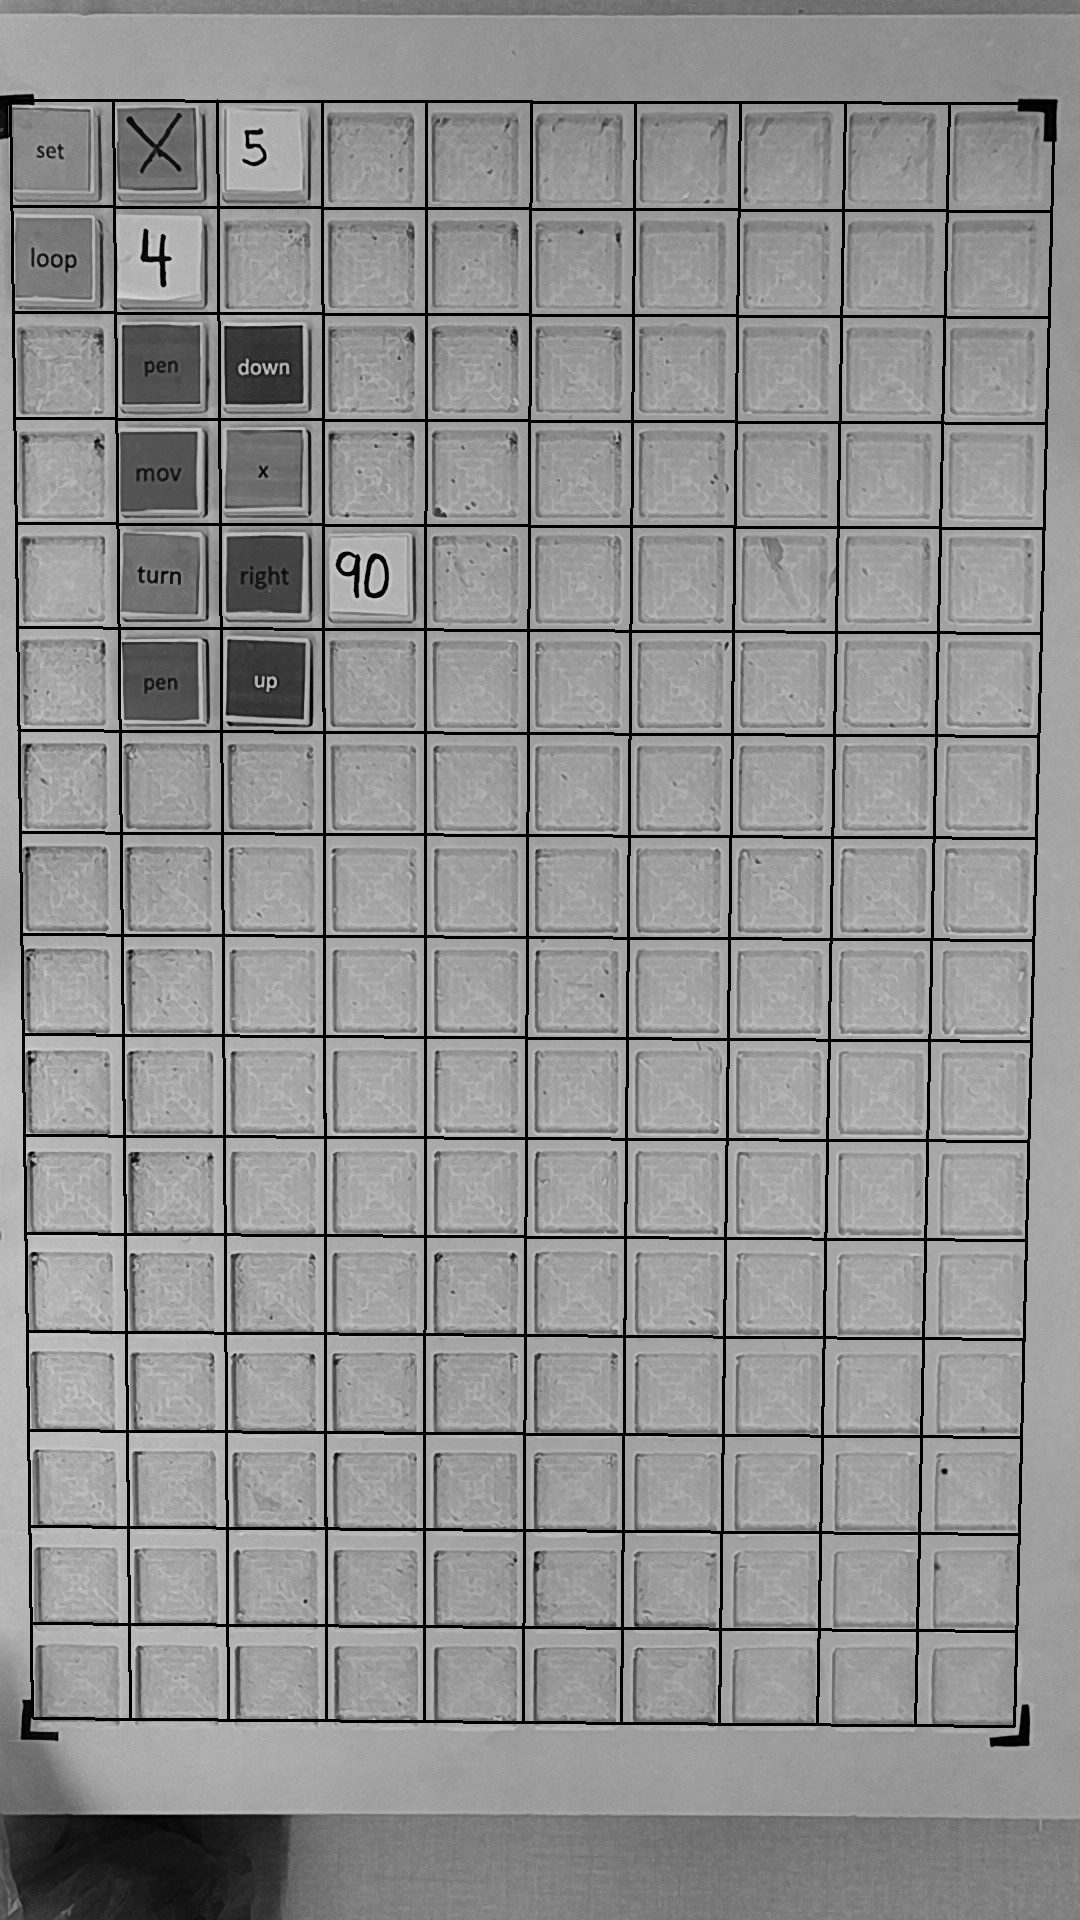
\includegraphics[width=0.8\textwidth]{assets/grid_overlay.jpg}
    \caption{Computer Vision Grid Detection and Perspective Transformation}
    \label{fig:grid_overlay}
\end{figure}

\subsubsection{Computer Vision System}
\textbf{Camera Setup}:
\begin{itemize}
    \item \textbf{OAK-D Camera}: High-resolution overhead mounting for complete grid visibility
    \item \textbf{Perspective Correction}: Automatic corner detection and transformation
    \item \textbf{Lighting Optimization}: Controlled conditions for consistent OCR performance
    \item \textbf{Real-time Processing}: Live image capture and processing capabilities
\end{itemize}

\subsection{Control Station}

\textbf{Raspberry Pi 4 Specifications}:
\begin{itemize}
    \item \textbf{Processing Power}: 2GB RAM for computer vision and real-time processing
    \item \textbf{Storage}: 32GB microSD card for system software and data
    \item \textbf{Connectivity}: WiFi for car communication, USB for camera interface
    \item \textbf{Display Interface}: Tablet integration for system status and control
\end{itemize}

\section{Software Architecture and Implementation}

\subsection{Core Module}

The core module provides foundational infrastructure with zero dependencies on other components, implementing clean architecture principles.

\subsubsection{WebSocket Server Implementation}
\begin{itemize}
    \item \textbf{Asynchronous Architecture}: Built on asyncio for concurrent client handling
    \item \textbf{JSON Protocol}: Structured command and response messaging
    \item \textbf{Broadcast Support}: System-wide notifications to all connected clients
    \item \textbf{Connection Management}: Automatic reconnection and error recovery
\end{itemize}

\subsubsection{Process Controller}
\begin{itemize}
    \item \textbf{Workflow Framework}: Generic execution pattern supporting any async function
    \item \textbf{Cancellation Support}: Clean cancellation through callback mechanisms
    \item \textbf{Progress Reporting}: Real-time status updates via message callbacks
    \item \textbf{Return Value Chaining}: Support for workflow data passing and composition
\end{itemize}

\subsubsection{Configuration Management}
\begin{itemize}
    \item \textbf{Pydantic Models}: Type-safe configuration with automatic validation
    \item \textbf{Environment Variables}: Flexible deployment configuration
    \item \textbf{Immutable Design}: Thread-safe configuration access
    \item \textbf{Default Values}: Comprehensive fallback configuration
\end{itemize}

\subsection{Vision Module}

The vision module handles the complete pipeline from image capture to structured grid data.

\subsubsection{Image Processing Pipeline}
\textbf{Multi-Source Capture}:
\begin{itemize}
    \item \textbf{Local Capture}: Direct OpenCV camera access for development
    \item \textbf{Remote Capture}: Client-server architecture for Raspberry Pi deployment
    \item \textbf{File Processing}: Static image testing and validation capabilities
    \item \textbf{Format Optimization}: Automatic rotation, scaling, and format conversion
\end{itemize}

\textbf{Grid Detection and Transformation}:
\begin{itemize}
    \item \textbf{Perspective Correction}: Homography transformation using configurable corner points
    \item \textbf{Grid Cell Mapping}: Precise boundary calculation for block position detection
    \item \textbf{Adaptive Scaling}: Support for different grid sizes and camera positions
    \item \textbf{Quality Validation}: Image quality assessment and optimization
\end{itemize}

\subsubsection{OCR Processing}
\textbf{EasyOCR Integration}:
\begin{itemize}
    \item \textbf{GPU Acceleration}: Hardware acceleration when available for improved performance
    \item \textbf{Confidence Scoring}: Recognition quality assessment for filtering
    \item \textbf{Bounding Box Detection}: Precise text localization within grid cells
    \item \textbf{Multi-language Support}: Optimized for English with extensibility
\end{itemize}

\subsubsection{OCR2Grid Mapping}
\textbf{Spatial Analysis}:
\begin{itemize}
    \item \textbf{Grid Association}: Geometric analysis to map detected text to specific grid positions
    \item \textbf{Confidence Filtering}: Elimination of false positives based on recognition confidence
    \item \textbf{Multi-word Support}: Handling of complex commands spanning multiple detection regions
    \item \textbf{Empty Cell Detection}: Proper handling of unoccupied grid positions
\end{itemize}

\subsection{Engine Module}

The engine module implements a comprehensive programming language interpreter using modern design patterns.

\subsubsection{Command System Architecture}
\textbf{Command Registry and Factory}:
\begin{itemize}
    \item \textbf{Dynamic Registration}: Automatic command discovery through module imports
    \item \textbf{Type Safety}: Parameter validation and type checking for all commands
    \item \textbf{Extensibility}: Plugin-style architecture for adding new commands
    \item \textbf{Error Handling}: Comprehensive validation and error reporting
\end{itemize}

\textbf{Parser Implementation}:
\begin{itemize}
    \item \textbf{Grid Traversal}: Left-to-right, top-to-bottom reading order
    \item \textbf{Indentation Scoping}: Column-based nesting similar to Python syntax
    \item \textbf{Special Cases}: Proper ELSE handling at matching indentation levels
    \item \textbf{Command Tree}: Hierarchical structure preserving execution order and nesting
\end{itemize}

\subsubsection{Programming Language Features}
\textbf{Movement Commands}:
\begin{itemize}
    \item \textbf{MOVE}: Forward/backward movement with distance parameters and sensor integration
    \item \textbf{TURN}: Directional rotation with degree specifications and conditional execution
    \item \textbf{WAIT}: Time-based pauses with conditional waiting capabilities
\end{itemize}

\textbf{Control Flow Constructs}:
\begin{itemize}
    \item \textbf{LOOP}: Count-based, conditional, and infinite loops with proper nesting
    \item \textbf{IF/ELSE}: Conditional execution with complex boolean expressions
    \item \textbf{WHILE}: Dynamic conditional loops with real-time sensor evaluation
\end{itemize}

\textbf{Data Manipulation}:
\begin{itemize}
    \item \textbf{SET}: Variable assignment with arithmetic and logical operations
    \item \textbf{Variables}: Named storage supporting numeric and boolean values
    \item \textbf{Expressions}: Mathematical operations with operator precedence and type coercion
\end{itemize}

\textbf{Sensor Integration}:
\begin{itemize}
    \item \textbf{DISTANCE}: Real-time ultrasonic sensor readings
    \item \textbf{OBSTACLE}: Boolean obstacle detection with configurable thresholds
    \item \textbf{BLACK\_DETECTED/BLACK\_LOST}: IR sensor integration for line following
\end{itemize}

\subsubsection{Value System and Expression Evaluation}
\textbf{Type System}:
\begin{itemize}
    \item \textbf{Number}: Integer and floating-point values with automatic conversion
    \item \textbf{Boolean}: Logical values with proper truth evaluation
    \item \textbf{Variable}: Dynamic typing with scope management
    \item \textbf{Direction}: Spatial orientation values (LEFT, RIGHT, FORWARD, BACKWARD)
    \item \textbf{Sensor}: Real-time sensor data access with caching
\end{itemize}

\textbf{Expression Processing}:
\begin{itemize}
    \item \textbf{Operator Support}: Arithmetic (+, -, *, /), comparison (<, >, =, !=), logical (AND, OR, NOT)
    \item \textbf{Left-to-Right Evaluation}: Consistent evaluation order with proper precedence
    \item \textbf{Type Coercion}: Automatic type conversion for mixed operations
    \item \textbf{Short-Circuit Evaluation}: Optimized logical operation processing
\end{itemize}

\subsubsection{Execution Context}
\textbf{State Management}:
\begin{itemize}
    \item \textbf{Position Tracking}: Coordinate system for car location and orientation
    \item \textbf{Variable Storage}: Scoped variable management with proper lifecycle
    \item \textbf{Drawing State}: Pen position and path tracking for creative tasks
    \item \textbf{Execution Limits}: Step counting and timeout protection
    \item \textbf{Path History}: Movement recording for visualization and debugging
\end{itemize}

\section{Arduino Firmware Implementation}

\subsection{Class-Based Architecture}

The Arduino firmware implements a sophisticated object-oriented design for maintainable and extensible hardware control.

\subsubsection{Core Classes}
\textbf{Motor Class}:
\begin{itemize}
    \item Direct hardware abstraction for individual motor control
    \item PWM speed control with direction management
    \item Consistent interface for all motor operations
\end{itemize}

\textbf{MotionController Class}:
\begin{itemize}
    \item High-level movement coordination using motor instances
    \item Sophisticated algorithms split across multiple files for organization
    \item Integration with sensor feedback for precise control
\end{itemize}

\textbf{GyroSensor Class}:
\begin{itemize}
    \item MPU-6050 integration with calibration and filtering
    \item Real-time orientation tracking and yaw calculation
    \item Temperature compensation and drift correction
\end{itemize}

\textbf{UltrasonicSensor Class}:
\begin{itemize}
    \item HC-SR04 distance measurement with noise filtering
    \item Configurable detection thresholds and timing
    \item Integration with movement algorithms for obstacle avoidance
\end{itemize}

\textbf{PenController Class}:
\begin{itemize}
    \item Servo-based pen positioning with smooth movement
    \item Position feedback and calibration support
    \item Integration with drawing coordinate system
\end{itemize}

\subsection{Advanced Movement Algorithms}

\subsubsection{Translation Control}
\textbf{Yaw Correction}:
\begin{itemize}
    \item Gyroscope-based straight-line movement compensation
    \item Real-time correction for motor imbalances and surface irregularities
    \item Configurable correction strength and response time
\end{itemize}

\textbf{Distance Calculation}:
\begin{itemize}
    \item Wheel circumference and gear ratio compensation
    \item Time-based movement with precise speed control
    \item Integration with encoder feedback when available
\end{itemize}

\subsubsection{Rotation Control}
\textbf{PID-Based Turning}:
\begin{itemize}
    \item Feedback control system for accurate angle achievement
    \item Direction change tracking for complex maneuvers
    \item Smooth acceleration and deceleration profiles
\end{itemize}

\textbf{Absolute and Relative Positioning}:
\begin{itemize}
    \item Support for both relative turns and absolute heading commands
    \item Reference orientation management and calibration
    \item Integration with global coordinate system
\end{itemize}

\begin{figure}[H]
    \centering
    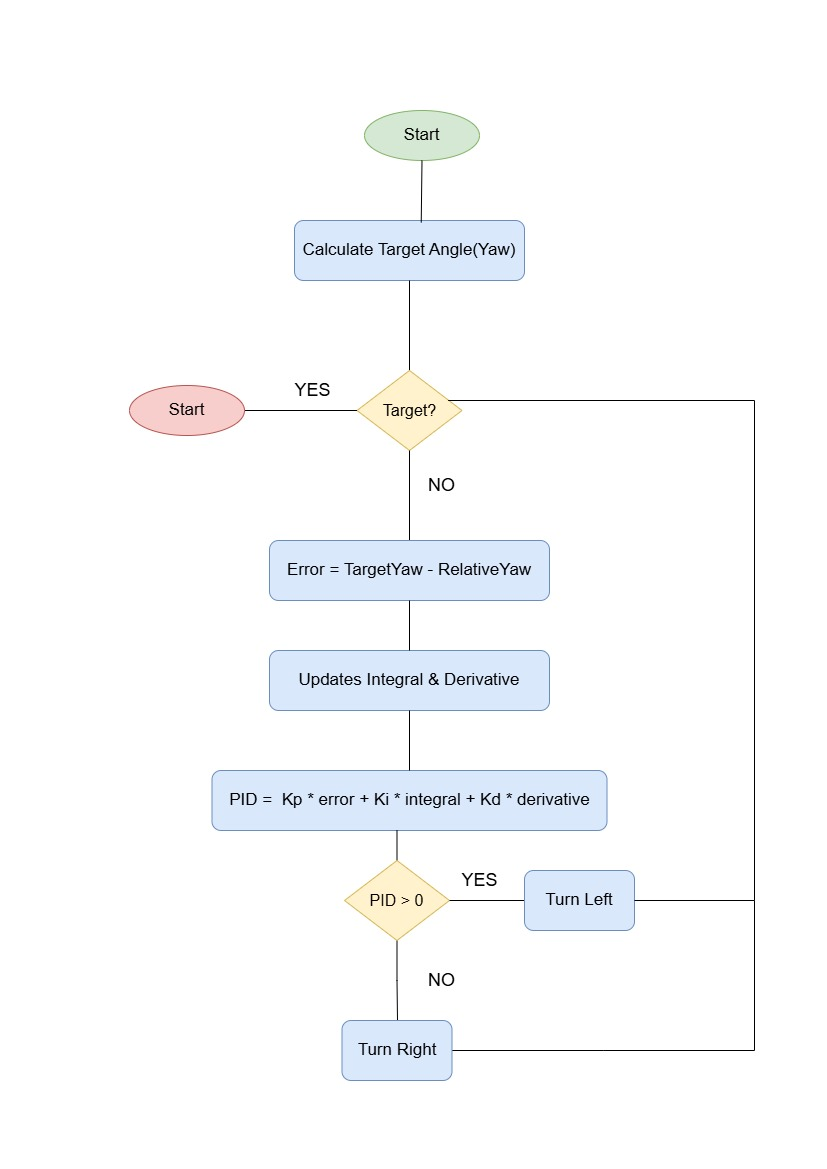
\includegraphics[width=0.7\textwidth]{assets/pid_algo_rotate.jpg}
    \caption{PID-Based Rotation Control Algorithm}
    \label{fig:pid_rotation}
\end{figure}

\subsection{Serial API Implementation}

\textbf{Command Protocol}:
\begin{itemize}
    \item JSON-based command format: \texttt{command:\{"param":"value"\}}
    \item Comprehensive parameter validation and error reporting
    \item Structured response format with success/failure indication
    \item Support for complex parameter combinations and optional values
\end{itemize}

\textbf{API Endpoints}:
\begin{itemize}
    \item \textbf{move}: Movement with speed, distance, and time parameters
    \item \textbf{rotate}: Rotation with angle, speed, and absolute positioning
    \item \textbf{pen}: Drawing control with position and action commands
    \item \textbf{gyro}: Sensor calibration and data access
    \item \textbf{sensor}: Distance measurement and obstacle detection
\end{itemize}

\section{Mobile Application Implementation}

\subsection{React Native Architecture}

\textbf{Framework and Platform}:
\begin{itemize}
    \item \textbf{React Native Expo}: Cross-platform development with native performance
    \item \textbf{iOS and Android}: Responsive design optimized for both platforms
    \item \textbf{WebSocket Integration}: Real-time communication with Raspberry Pi
    \item \textbf{Modern UI}: Built-in React Native components with smooth animations
\end{itemize}

\subsection{User Interface Design}

\textbf{Welcome Screen}:
\begin{itemize}
    \item Animated logo with professional design
    \item Modern solid color backgrounds with decorative elements
    \item Smooth transitions and call-to-action buttons
\end{itemize}

\textbf{Chat Interface}:
\begin{itemize}
    \item Real-time messaging with WebSocket server on Raspberry Pi
    \item Connection status indicators with pulsing animations
    \item Dedicated Run/Stop action buttons for program execution
    \item Markdown support for rich text rendering of system responses
    \item Auto-scroll functionality for latest message visibility
\end{itemize}

\textbf{Communication Features}:
\begin{itemize}
    \item JSON message protocol for command and status exchange
    \item Error handling and connection recovery mechanisms
    \item Message queuing for reliable delivery
    \item Real-time status updates and execution progress monitoring
\end{itemize}

\section{Development Methodology}

\subsection{Iterative Development Process}

The system was developed using an iterative approach with continuous integration and testing:

\subsubsection{Phase-Based Development}
\textbf{Phase 1 - Core Infrastructure}: WebSocket server, process control, and basic communication protocols

\textbf{Phase 2 - Computer Vision}: Camera integration, OCR processing, and grid mapping algorithms

\textbf{Phase 3 - Command Interpreter}: Programming language design, parser implementation, and execution engine

\textbf{Phase 4 - Hardware Integration}: Arduino firmware, ESP32 bridge, and sensor calibration

\textbf{Phase 5 - Mobile Application}: User interface development and WebSocket communication integration

\subsection{Testing and Validation}

\textbf{Component Testing}:
\begin{itemize}
    \item Unit tests for individual modules and classes
    \item Integration tests for communication protocols
    \item Hardware-in-the-loop testing for robotic components
    \item End-to-end workflow validation
\end{itemize}

\textbf{Performance Validation}:
\begin{itemize}
    \item Image processing performance under 2 seconds for block recognition
    \item Real-time program execution with immediate response
    \item Sub-100ms latency for car movement commands
    \item Reliable operation under classroom conditions
\end{itemize}

\section{System Integration and Deployment}

\subsection{Communication Protocols}

\textbf{WebSocket Communication}:
\begin{itemize}
    \item Real-time bidirectional communication between Raspberry Pi and mobile app
    \item JSON message format for commands and status updates
    \item Broadcast support for multiple connected clients
    \item Automatic reconnection and error recovery
\end{itemize}

\textbf{HTTP REST API}:
\begin{itemize}
    \item ESP32-hosted API for car control operations
    \item Stateless design for reliable remote operation
    \item Comprehensive error reporting with HTTP status codes
    \item Timeout management and retry mechanisms
\end{itemize}

\textbf{Serial Communication}:
\begin{itemize}
    \item 115200 baud UART between ESP32 and Arduino
    \item JSON protocol for command translation
    \item Flow control and error detection
    \item Command validation and response formatting
\end{itemize}

\subsection{Deployment Considerations}

\textbf{Classroom Requirements}:
\begin{itemize}
    \item Portable setup with minimal technical requirements
    \item Robust operation under variable lighting conditions
    \item Simple startup and shutdown procedures
    \item User-friendly error messages and recovery options
\end{itemize}

\textbf{Scalability Features}:
\begin{itemize}
    \item Configurable grid sizes for different complexity levels
    \item Extensible command system for curriculum adaptation
    \item Multiple car support for collaborative projects
    \item Modular architecture enabling component upgrades
\end{itemize}

The implementation successfully delivers a comprehensive educational system that integrates multiple technologies into a cohesive, engaging learning platform. The modular architecture ensures maintainability and extensibility while the robust communication protocols provide reliable operation in educational environments.

\begin{figure}[H]
    \centering
    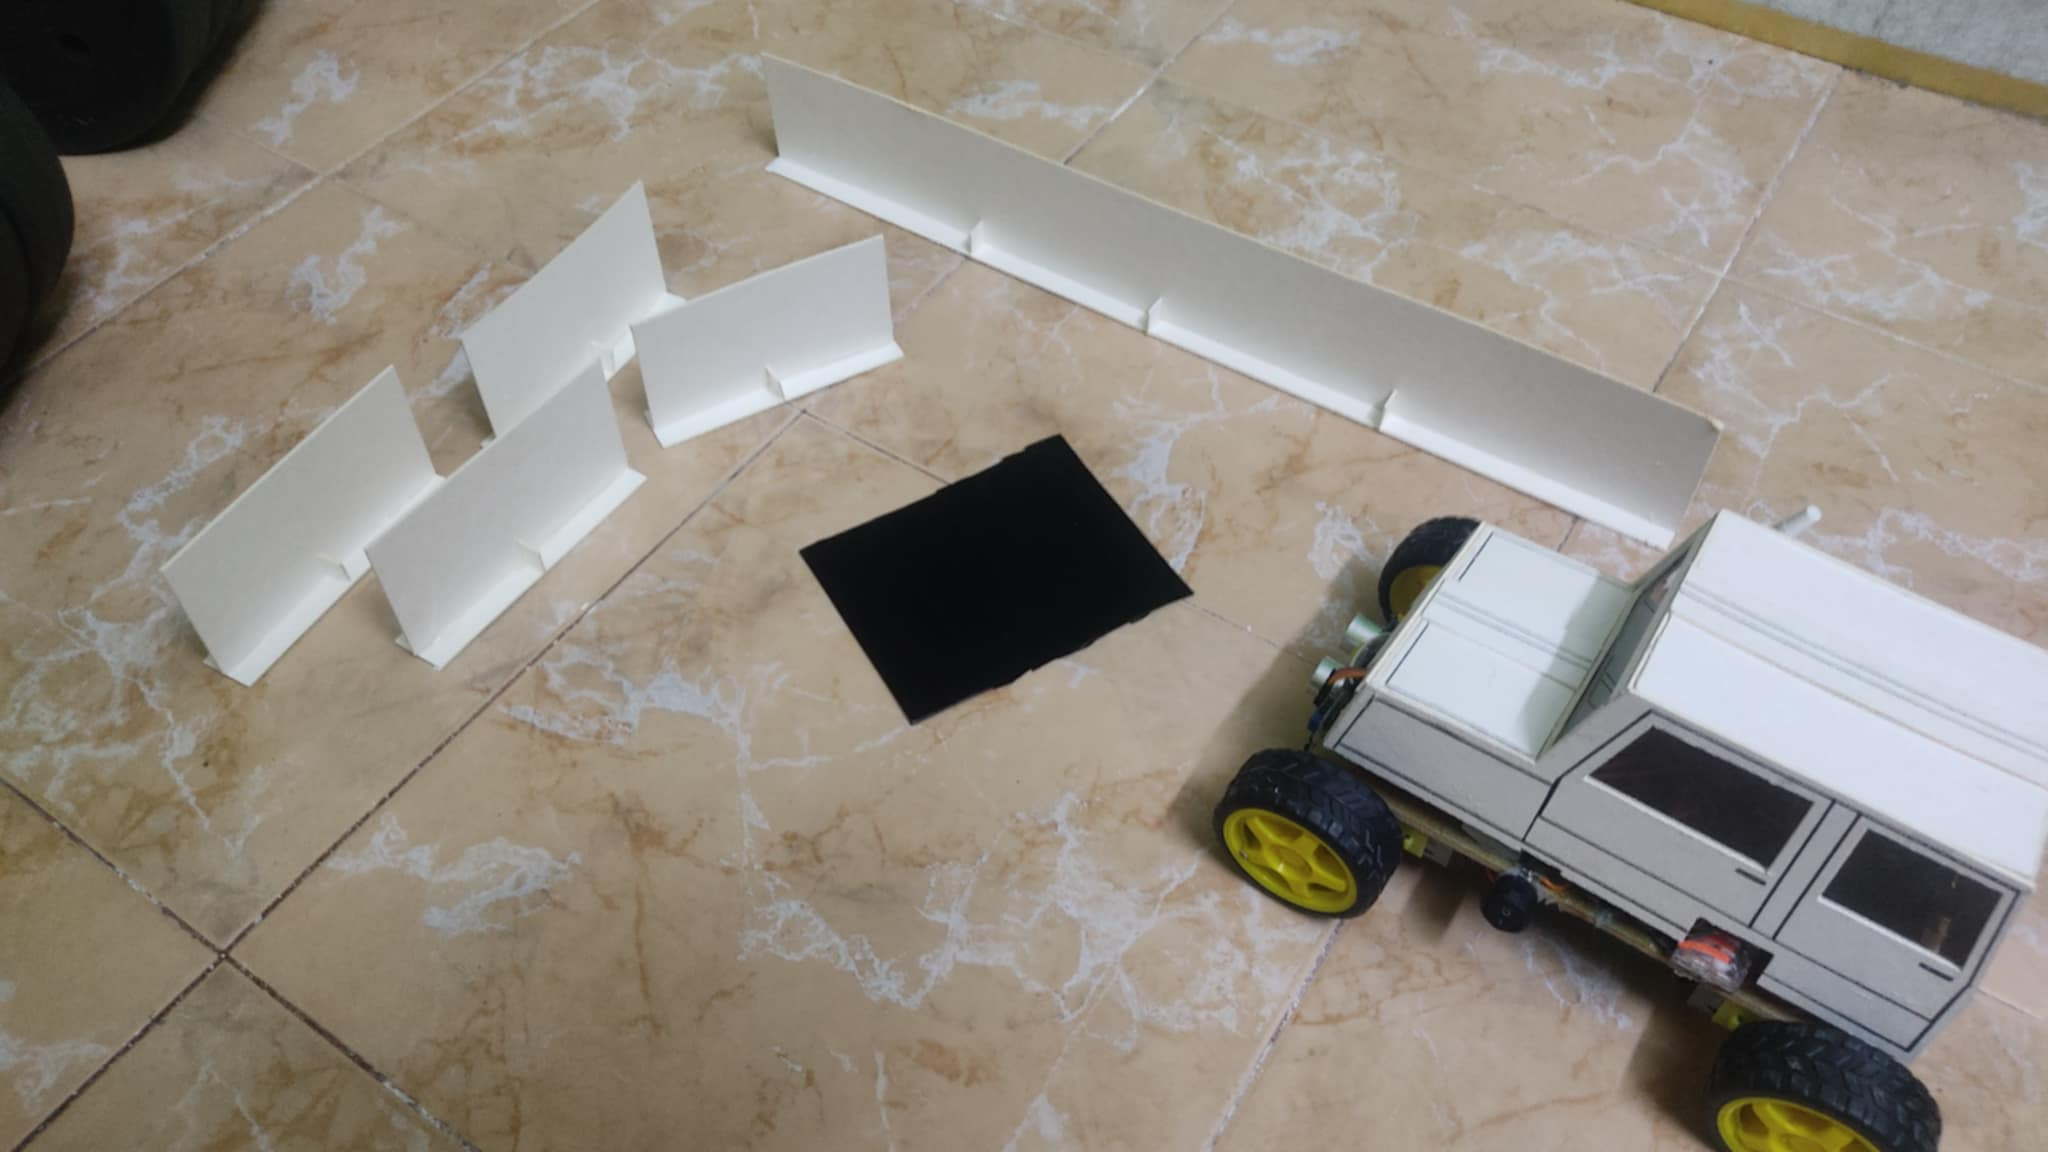
\includegraphics[width=0.8\textwidth]{assets/car_and_walls.png}
    \caption{TinkerBlocks Car with Obstacle Used in Gameplay}
    \label{fig:car_obstacles}
\end{figure}